\chapter{Вставка, обновление и удаление данных}

\section{Вставка данных}

\subsection{Инструкция INSERT VALUES}

\begin{lstlisting}[label=lst:funcReturn, language=sql]
	INSERT INTO Sales.MyOrders(custid, empid, orderdate, shipcountry, freight)
	VALUES(2, 19, '20120620', N'USA', 30.00);
\end{lstlisting}

Указание имен целевых столбцов после имени таблицы является необязательным,
но считается наиболее правильным.


\begin{lstlisting}[label=lst:funcReturn, language=sql]
	INSERT INTO Sales.MyOrders(custid, empid, orderdate, shipcountry, freight)
	VALUES(3, 17, DEFAULT, N'USA', 30.00); 
\end{lstlisting}

Если значение для столбца не задано, SQL Server сначала проверит, получает ли
столбец свое значение автоматически, например, с помощью свойства IDENTITY или
ограничения по умолчанию. Если нет, SQL Server проверит, допускается ли
в столбце использование значений NULL, и если так, будет присвоено значение NULL.
Если и это невозможно, SQL Server сгенерирует ошибку.


\subsection{Инструкция INSERT SELECT}

\begin{lstlisting}[label=lst:funcReturn, language=sql]
	INSERT INTO Sales.MyOrders(orderid, custid, empid, orderdate, shipcountry, freight)
		SELECT orderid, custid, empid, orderdate, shipcountry, freight
 		FROM Sales.Orders
 		WHERE shipcountry = N'Norway';
\end{lstlisting}

\subsection{Инструкция INSERT EXEC}

\begin{lstlisting}[label=lst:funcReturn, language=sql]
	CREATE PROC Sales.OrdersForCountry @country AS NVARCHAR(15)
		AS
		SELECT orderid, custid, empid, orderdate, shipcountry, freight
		FROM Sales.Orders
		WHERE shipcountry = @country;

	INSERT INTO Sales.MyOrders(orderid, custid, empid, orderdate, shipcountry, freight)
 	EXEC Sales.OrdersForCountry
 	@country = N'Portugal';
\end{lstlisting}

\begin{figure}[h!]
	\begin{center}
		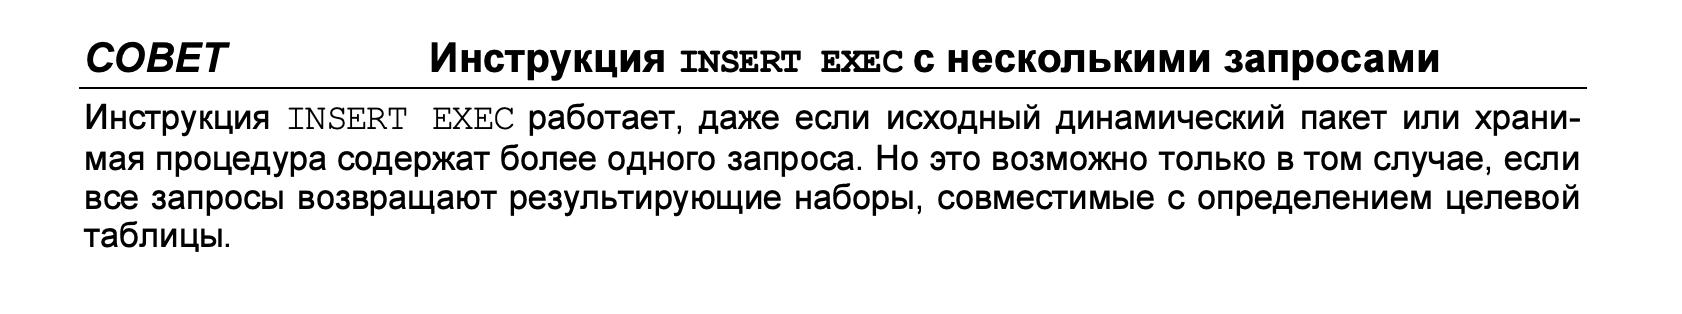
\includegraphics[width=0.9\textwidth]{img/advice21.png}
	\end{center}
	\captionsetup{justification=centering}
\end{figure}


\subsection{Инструкция SELECT INTO}

Эта инструкция создает целевую таблицу, опираясь на определение источника, и вставляет результирующие строки из запроса в эту таблицу.
Кроме самих данных, инструкция копирует из источника некоторые компоненты
определения данных, такие как имена столбцов, типы данных, возможность использования значения NULL и свойство IDENTITY.

\begin{lstlisting}[label=lst:funcReturn, language=sql]
	SELECT orderid, custid, orderdate, shipcountry, freight
	INTO Sales.MyOrders
	FROM Sales.Orders
	WHERE shipcountry = N'Norway';
\end{lstlisting}

Исходный столбец orderid имеет свойство IDENTITY, и, соответственно,
целевой столбец также определен со свойством IDENTITY. Если вы хотите, чтобы у целевого столбца не было этого свойства, вам следует выполнить некоторую обработку, например, orderid + 0 AS orderid.

сли необходимо, чтобы целевой столбец был определен как недопускающий значения NULL, требуется использовать функцию ISNULL: ISNULL(orderid + 0, -1) AS
orderid. 

Чтобы преобразовать исходный тип данных столбца
orderdate DATETIME в тип данных DATE в целевом столбце и отменить разрешение
значений NULL, используйте выражение ISNULL(CAST(orderdate AS DATE),
'19000101') AS orderdate. 

Помните, что инструкция SELECT INTO не копирует ограничения из исходной таблицы, поэтому, если они нужны, вы сами должны определить их в целевой таблице.
Например, следующий код определяет ограничение первичного ключа в целевой
таблице. 

\begin{figure}[h!]
	\begin{center}
		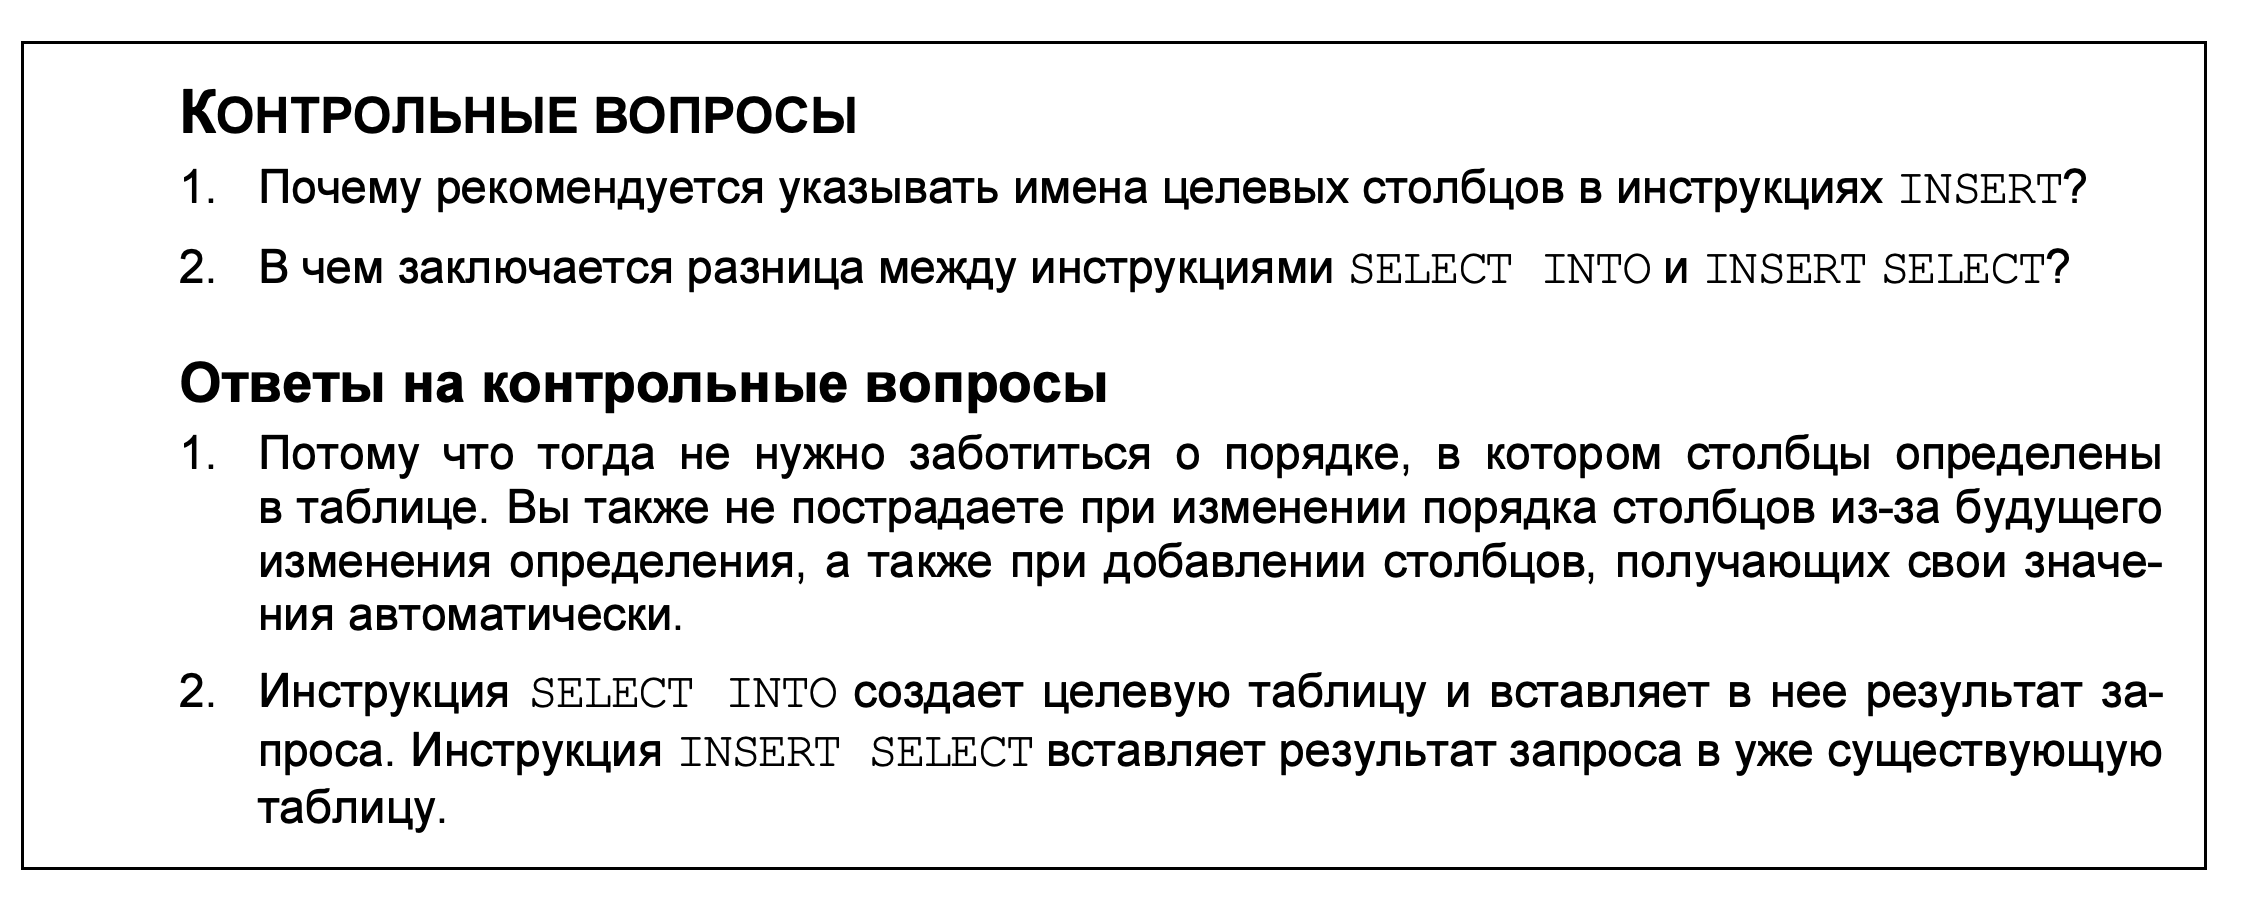
\includegraphics[width=0.9\textwidth]{img/control21.png}
	\end{center}
	\captionsetup{justification=centering}
\end{figure}


		
\subsection*{Резюме занятия}
\begin{itemize}
	\item Язык T-SQL поддерживает различные инструкции, выполняющие вставку данных в таблицы в базе данных. К ним относятся инструкции INSERT VALUES, INSERT
	SELECT, INSERT EXEC, SELECT INTO и др. 
	\item С помощью инструкции INSERT VALUES можно вставлять одну или более строк
	в целевую таблицу, опираясь на выражения значений. 
	\item С помощью инструкции INSERT SELECT можно вставлять в целевую таблицу результат запроса. 
	\item Можно использовать инструкцию INSERT EXEC для вставки в целевую таблицу
	результата запросов в динамическом пакете или хранимой процедуре.
	\item  Используя инструкции INSERT VALUES, INSERT SELECT и INSERT EXEC, можно опустить столбцы, получающие свои значения автоматически. Столбец может получить свое значение автоматически, если он имеет связанное с ним ограничение
	по умолчанию, или свойство IDENTITY, или если он допускает использование
	значений NULL.
	\item Инструкция SELECT INTO создает целевую таблицу на основании определения
	данных в исходном запросе и вставляет результат запроса в целевую таблицу. 
	\item Считается наиболее правильным указывать в инструкции INSERT имена целевых
	столбцов, чтобы удалить зависимость от порядка следования столбцов в определении целевой таблицы. 
\end{itemize}

\subsection*{Закрепление материала}

\begin{figure}[h!]
	\begin{center}
		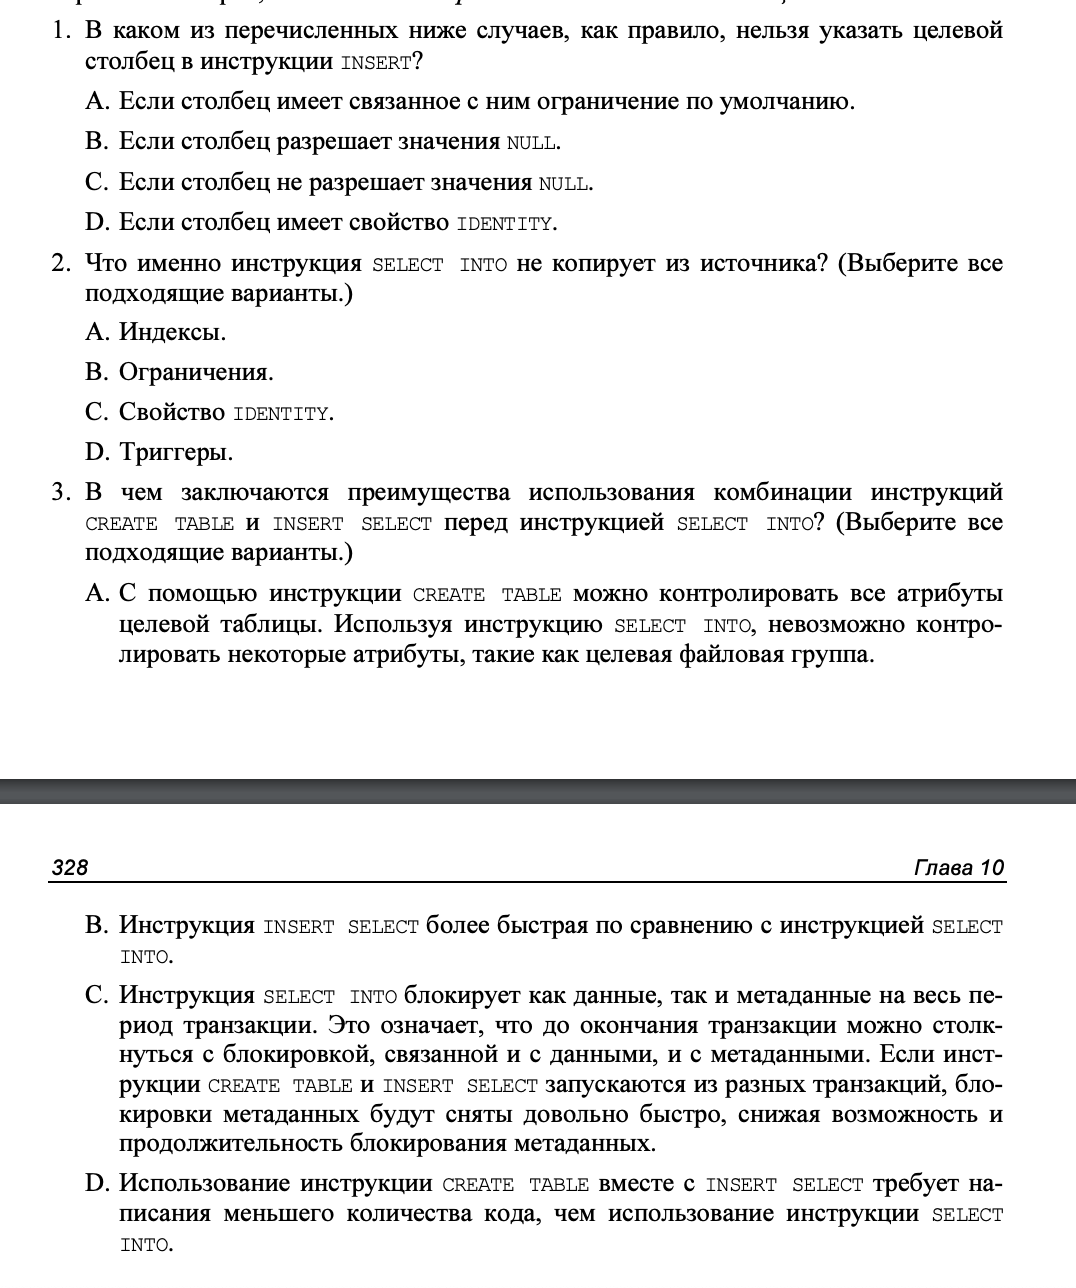
\includegraphics[width=0.9\textwidth]{img/zakrep20.png}
	\end{center}
	\captionsetup{justification=centering}
\end{figure}
\clearpage

\subsection*{Ответы}

\begin{figure}[h!]
	\begin{center}
		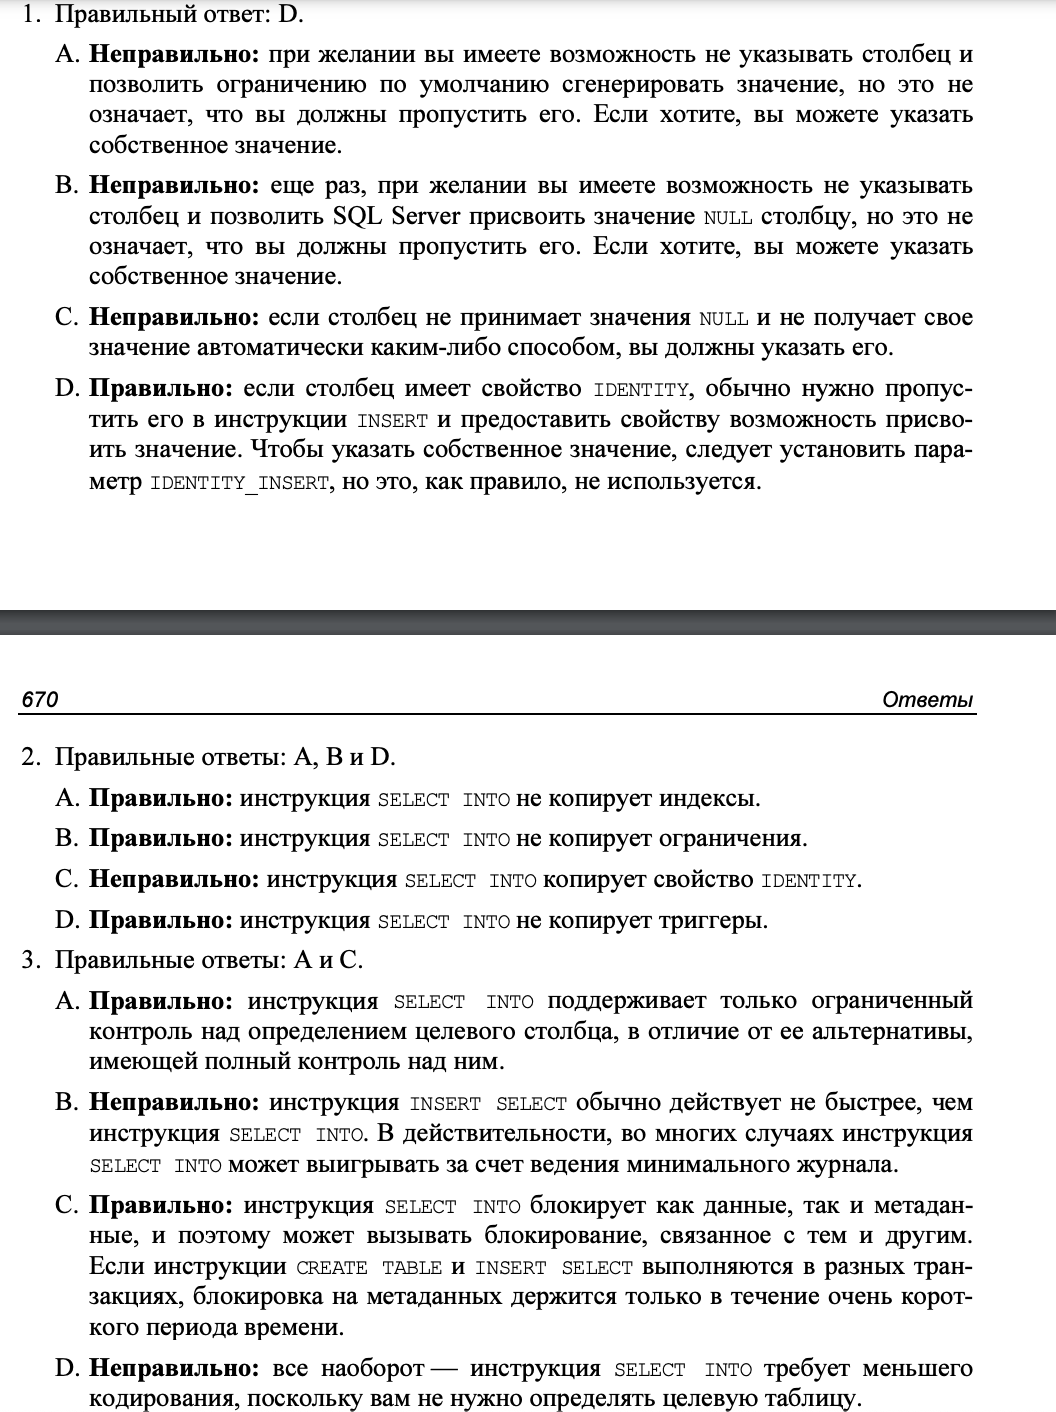
\includegraphics[width=0.9\textwidth]{img/ans21.png}
	\end{center}
	\captionsetup{justification=centering}
\end{figure}


\section{Обновление данных}

\subsection{Инструкция UPDATE}

\begin{lstlisting}[label=lst:funcReturn, language=sql]
	UPDATE <target table>
	SET <col 1> = <expression 1>,
	<col 2> = <expression 2>,
	..., <col n> = <expression n>
   WHERE <predicate>;
\end{lstlisting}

\subsection{Обновление с использованием объединения}

Стандартный язык SQL не поддерживает объединения в инструкции UPDATE, но
язык T-SQL поддерживает.

\begin{lstlisting}[label=lst:funcReturn, language=sql]
	UPDATE OD
	SET OD.discount += 0.05
   FROM Sales.MyCustomers AS C
	INNER JOIN Sales.MyOrders AS O
	ON C.custid = O.custid
	INNER JOIN Sales.MyOrderDetails AS OD
	ON O.orderid = OD.orderid
   WHERE C.country = N'Norway'; 
\end{lstlisting}


\subsection{Инструкция UPDATE и табличные выражения}

\begin{lstlisting}[label=lst:funcReturn, language=sql]
	WITH C AS
	(SELECT TGT.custid,
	 TGT.country AS tgt_country, SRC.country AS src_country,
	 TGT.postalcode AS tgt_postalcode, SRC.postalcode AS src_postalcode
	 FROM Sales.MyCustomers AS TGT
	 INNER JOIN Sales.Customers AS SRC
	 ON TGT.custid = SRC.custid )
	UPDATE C
	 SET tgt_country = src_country,
	 tgt_postalcode = src_postalcode;
\end{lstlisting}


\begin{figure}[h!]
	\begin{center}
		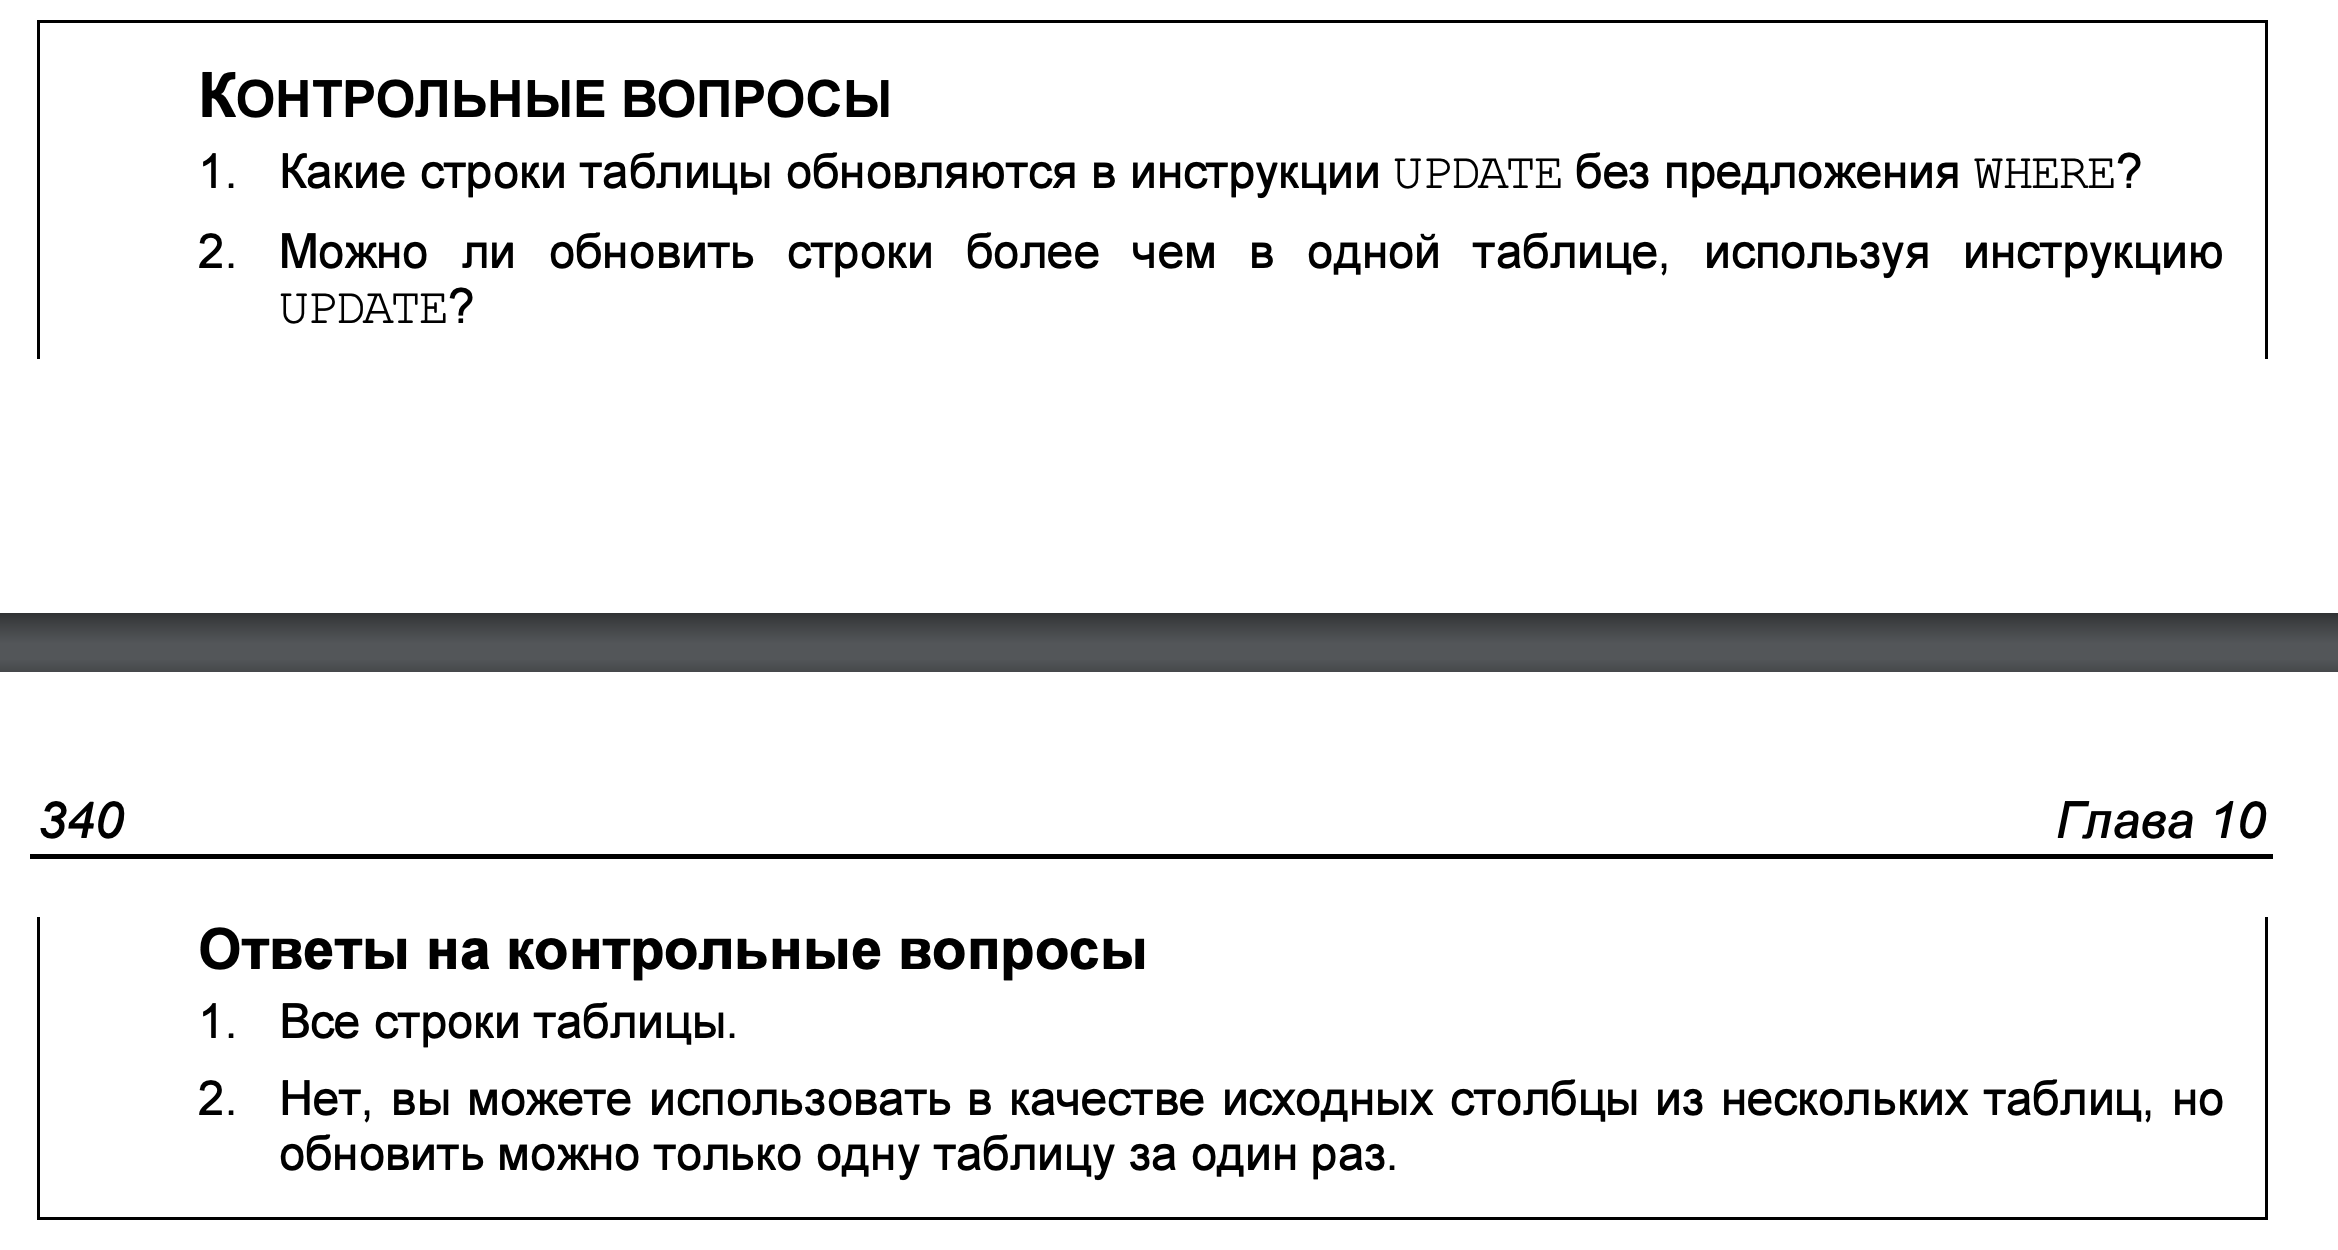
\includegraphics[width=0.9\textwidth]{img/control22.png}
	\end{center}
	\captionsetup{justification=centering}
\end{figure}



\subsection*{Резюме занятия}
\begin{itemize}
	\item Язык T-SQL поддерживает стандартную инструкцию UPDATE, а также несколько
	расширений к стандарту. 
	\item Вы можете изменить данные в одной таблице, используя данные другой таблицы, с помощью инструкции UPDATE на основе объединений. Но следует помнить,
	что если несколько исходных строк соответствуют одной целевой строке, обновление не приведет к ошибке; оно будет недетерминированным. В общем
	случае следует избегать таких обновлений. 
	\item T-SQL поддерживает обновление данных с помощью табличных выражений.
	Эта возможность удобна, когда вы хотите иметь возможность увидеть результат
	запроса до фактического обновления данных. Также это удобно, когда нужно
	изменить строки с помощью выражений, которые обычно запрещены в предложении SET, например оконных функций. 
	\item  Если вам нужно модифицировать строку и запросить результат этого изменения,
	можно использовать специализированную инструкцию UPDATE с переменной, которая может выполнить это за одно обращение к строке. 
\end{itemize}


\subsection*{Закрепление материала}

\begin{figure}[h!]
	\begin{center}
		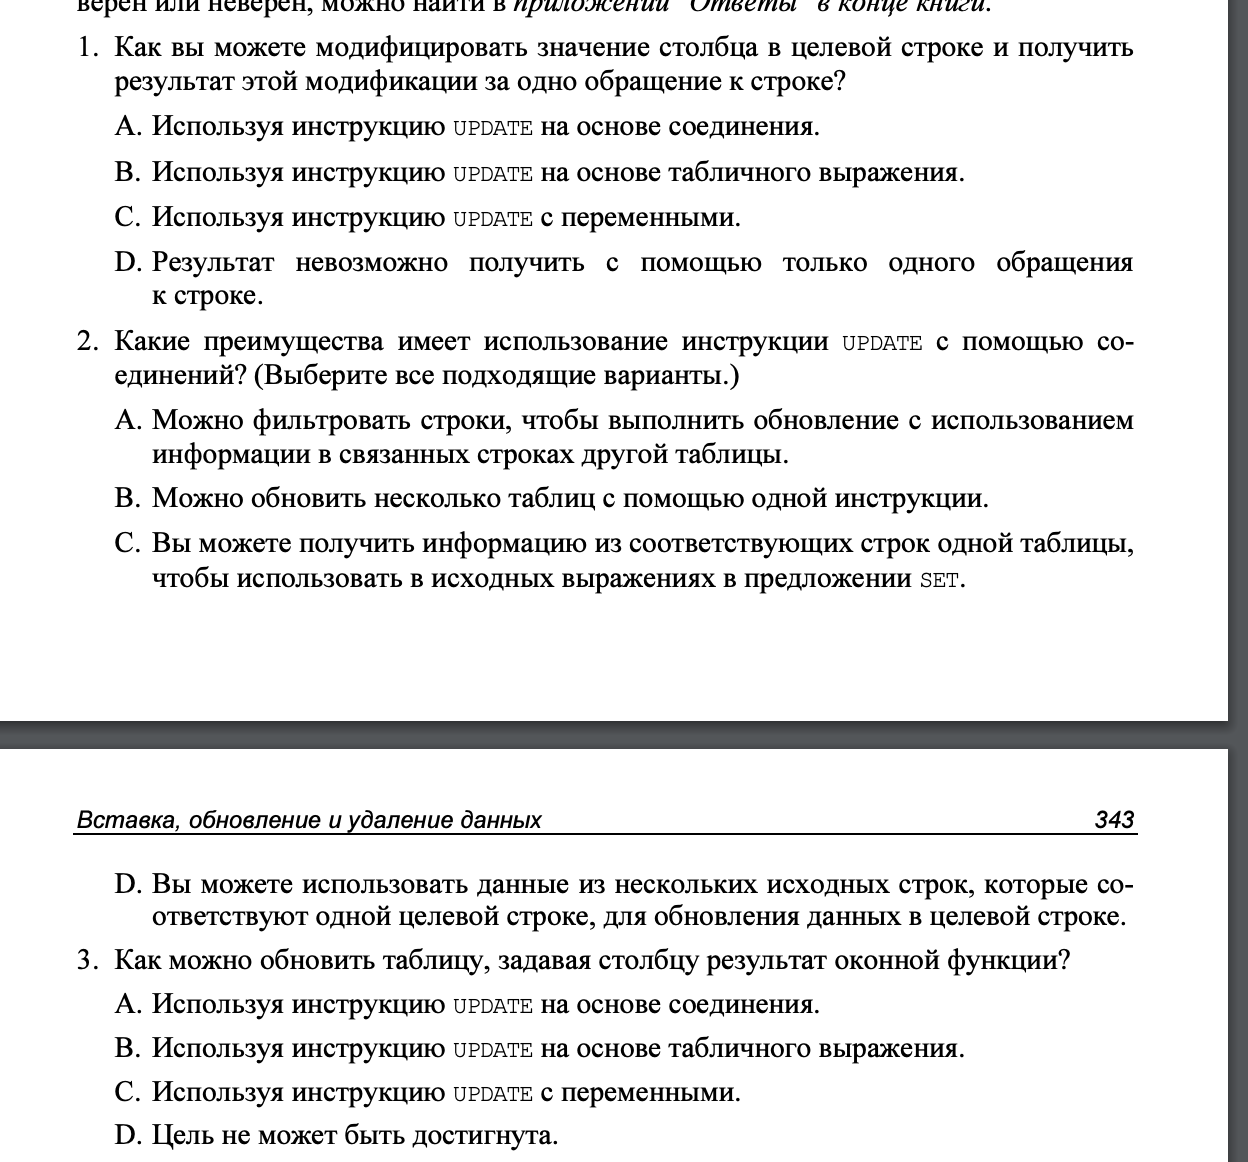
\includegraphics[width=0.9\textwidth]{img/zakrep21.png}
	\end{center}
	\captionsetup{justification=centering}
\end{figure}
\clearpage

\subsection*{Ответы}

\begin{figure}[h!]
	\begin{center}
		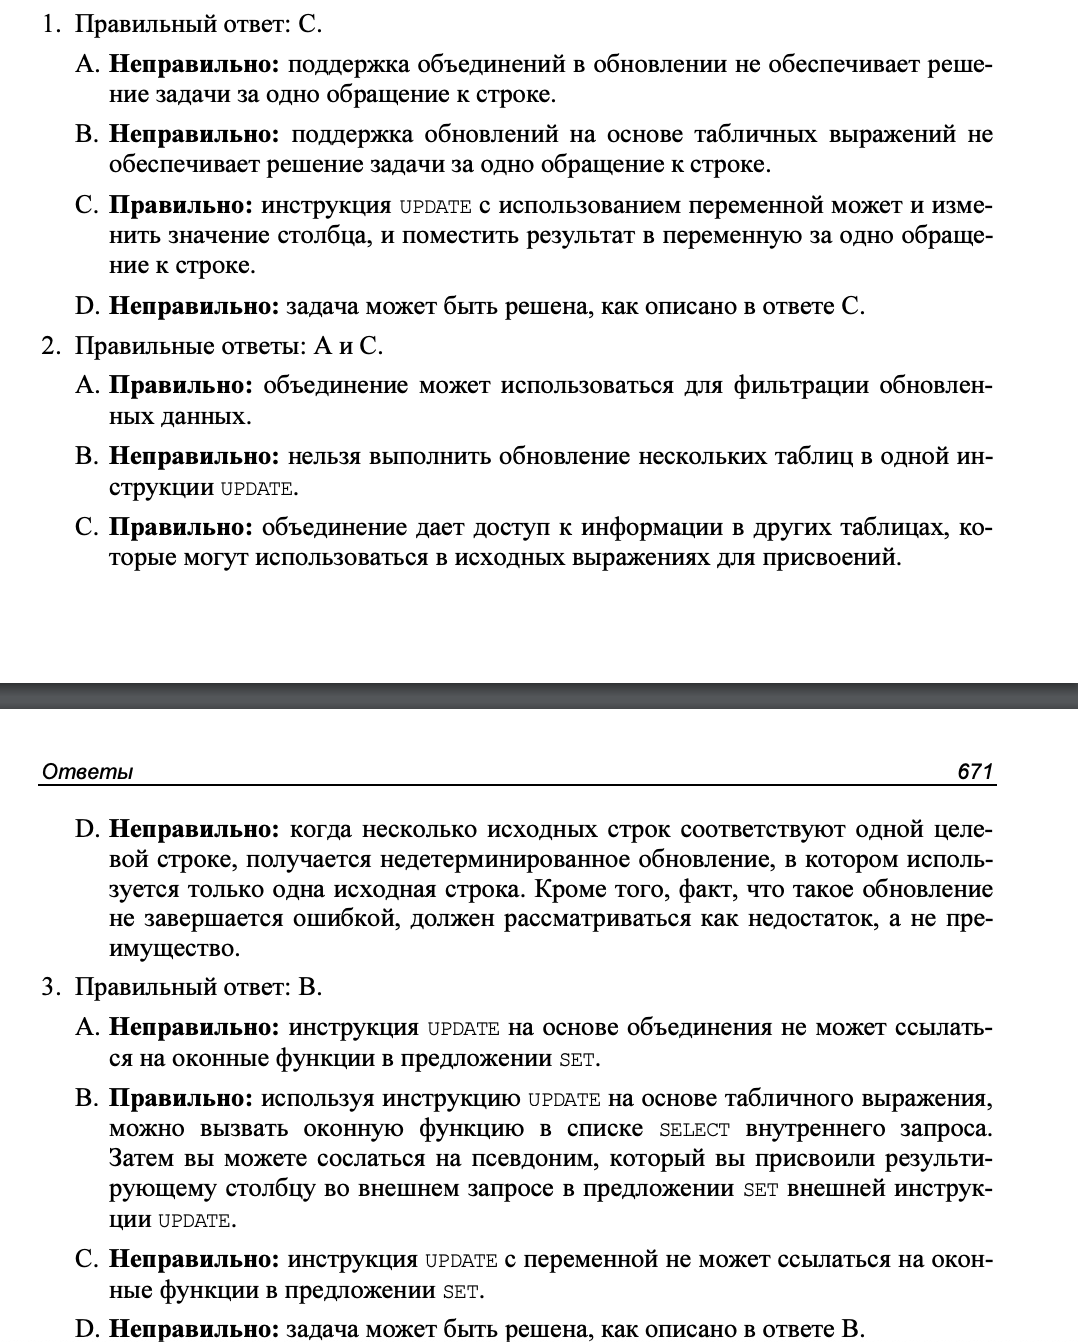
\includegraphics[width=0.8\textwidth]{img/ans22.png}
	\end{center}
	\captionsetup{justification=centering}
\end{figure}




\section{Удаление данных}

\subsection{Инструкция DELETE}

Инструкция
DELETE выполняется с полным протоколированием, и, следовательно, удаление
большого количества данных может требовать много времени для своего завершения. Такие объемные удаления могут приводить к значительному увеличению журнала транзакций. Они также могут приводить к укрупнению блокировок, а это означает, что SQL Server укрупняет блокировки мелких фрагментов данных, такие
как блокировки строк, до полной блокировки таблицы.

Решением может послужить следующий пример:



\begin{lstlisting}[label=lst:funcReturn, language=sql]
	WHILE 1 = 1
	BEGIN
	 DELETE TOP (1000) FROM Sales.MyOrderDetails
	 WHERE productid = 12;
	 IF @@rowcount < 1000 BREAK;
	END 
\end{lstlisting}

\subsection{Инструкция TRUNCATE}

Существует несколько важных различий между инструкцией DELETE и инструкцией
TRUNCATE. 

\begin{itemize}
	\item Инструкция DELETE записывает в журнал транзакций значительно больше информации, чем инструкция TRUNCATE. В случае инструкции DELETE, SQL Server
	записывает в журнал реальные данные, которые были удалены. Для инструкции
	TRUNCATE SQL Server записывает только информацию о том, какие страницы были освобождены. В результате инструкция TRUNCATE выполняется существенно
	быстрее.
	\item Инструкция DELETE не пытается сбросить свойство идентификатора, если оно
	установлено для столбца в целевой таблице. Инструкция TRUNCATE делает это.
	Если вы используете инструкцию TRUNCATE и хотели бы не сбрасывать это свойство, вам необходимо сохранить текущее значение идентификатора в переменной (используя функцию IDENT\_CURRENT) и восстановить сохраненное значение
	свойства после усечения таблицы. 
	\item Инструкция DELETE поддерживается, если имеется внешний ключ, указывающий
	на запрашиваемую таблицу, при условии, что в ссылающейся таблице нет связанных строк. Инструкция TRUNCATE не разрешена, если внешний ключ указывает
	на таблицу — даже если в ссылающейся таблице нет связанных строк и даже
	если внешний ключ запрещен. 
	\item Инструкция DELETE применяется к таблице, являющейся частью индексированного представления. Инструкция TRUNCATE в таком случае является недопустимой. 
	\item Инструкция DELETE требует разрешений DELETE на целевую таблицу. Инструкция
	TRUNCATE требует разрешений ALTER на целевую таблицу. 
\end{itemize}

Если необходимо удалить все строки таблицы, обычно следует использовать инструкцию TRUNCATE, потому что она значительно быстрее инструкции DELETE. Однако
она требует больших разрешений и имеет больше ограничений. 


\subsection{Инструкция DELETE на основе объединений}

\begin{lstlisting}[label=lst:funcReturn, language=sql]
	DELETE FROM O
	FROM Sales.MyOrders AS O
	 INNER JOIN Sales.MyCustomers AS C
	 ON O.custid = C.custid
	WHERE C.country = N'USA';
\end{lstlisting}

Можно реализовать эту же задачу, используя вложенный запрос объединения, как
показано в следующем примере: 

\begin{lstlisting}[label=lst:funcReturn, language=sql]
	DELETE FROM Sales.MyOrders
	WHERE EXISTS
	( SELECT *
	 FROM Sales.MyCustomers
	 WHERE MyCustomers.custid = MyOrders.custid
	 AND MyCustomers.country = N'USA'); 
\end{lstlisting}

Эта инструкция оптимизируется так же, как инструкция, использующая объединение, поэтому, с точки зрения производительности, не существует предпочтения одной версии по сравнению с другой.


\subsection{Инструкция DELETE с табличными выражениями}

\begin{lstlisting}[label=lst:funcReturn, language=sql]
	WITH OldestOrders AS
	( SELECT TOP (100) *
	 FROM Sales.MyOrders
	 ORDER BY orderdate, ordered )
	DELETE FROM OldestOrders; 
\end{lstlisting}


\begin{figure}[h!]
	\begin{center}
		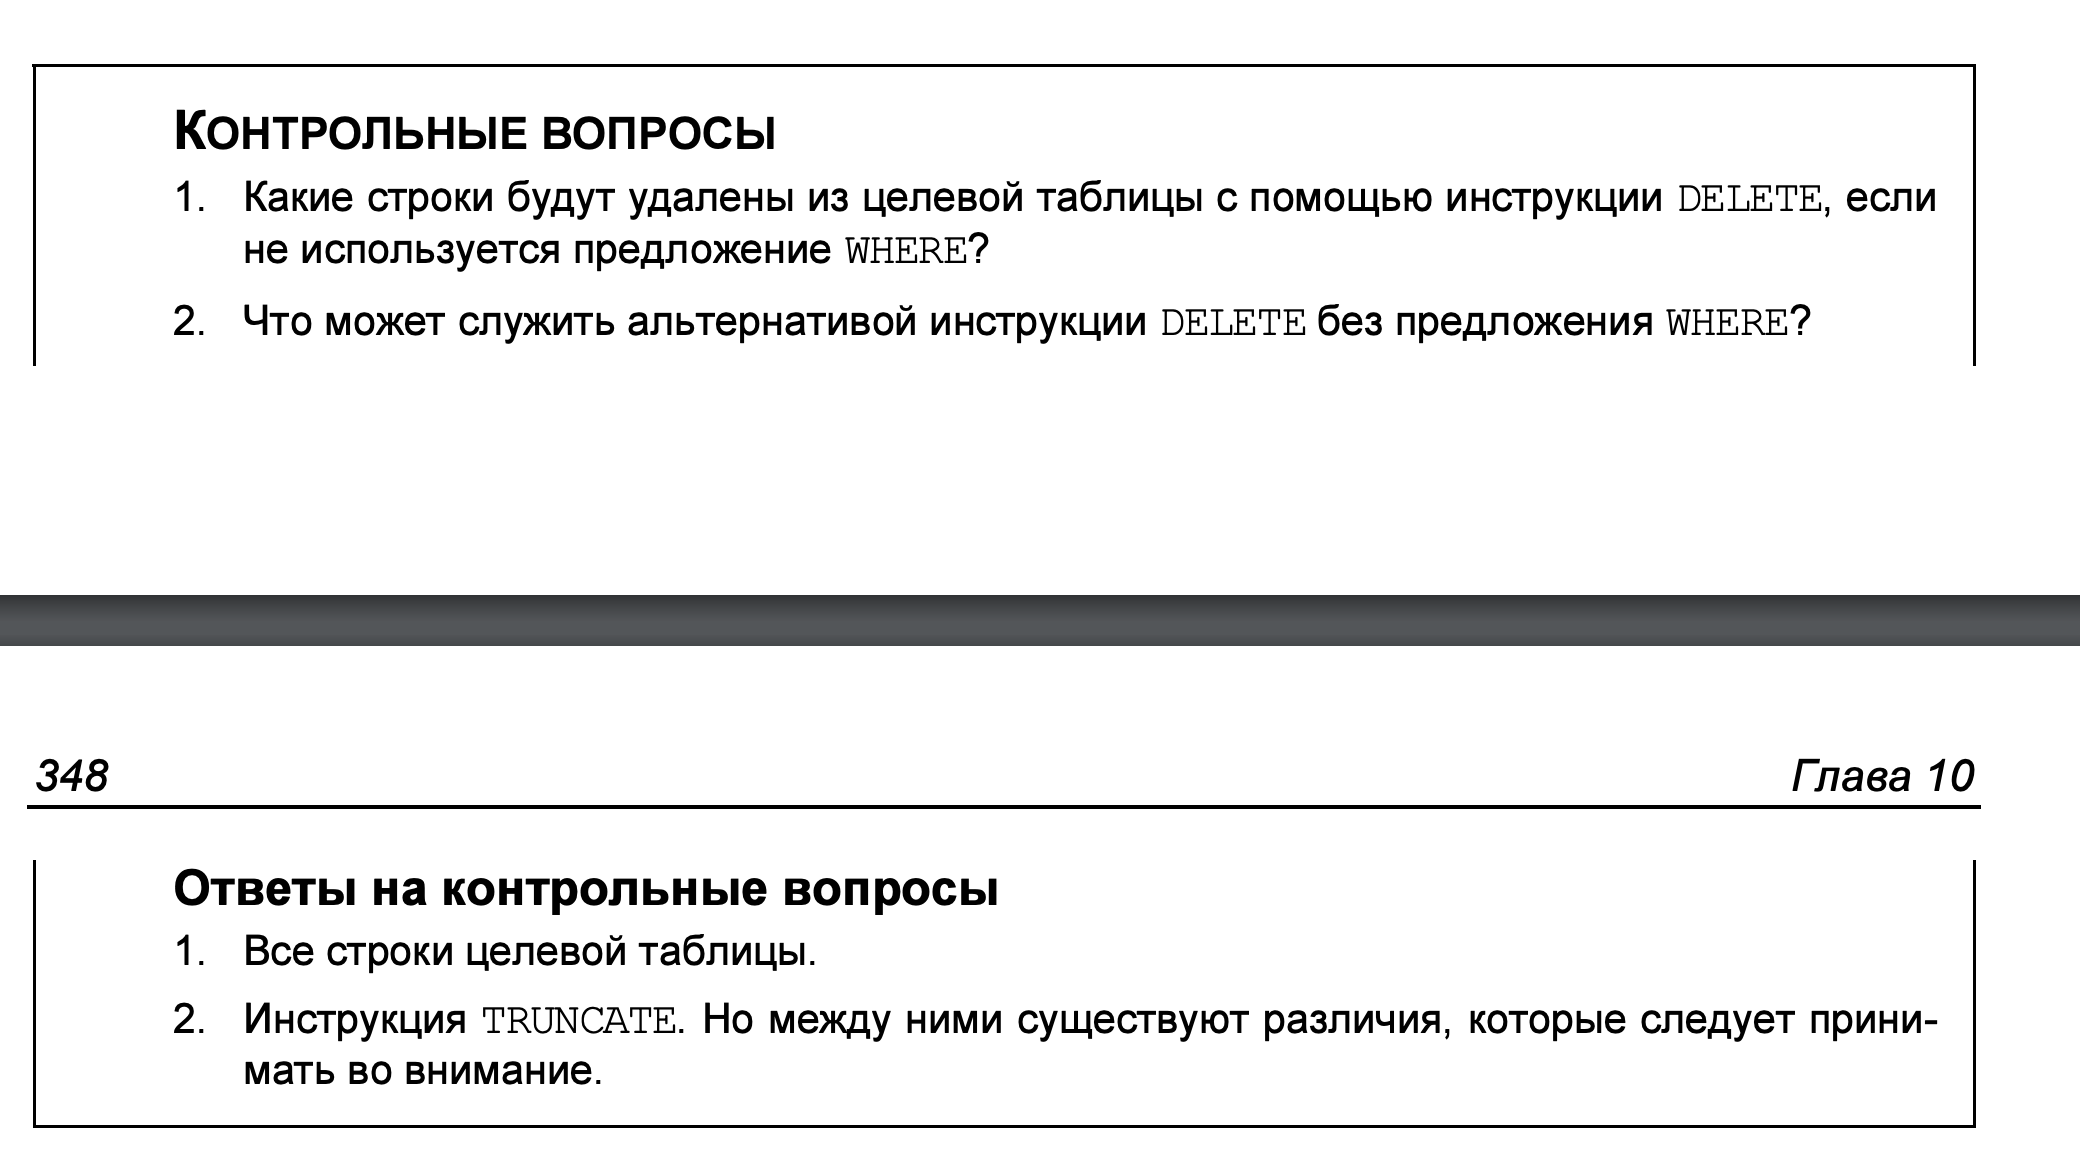
\includegraphics[width=0.8\textwidth]{img/control23.png}
	\end{center}
	\captionsetup{justification=centering}
\end{figure}



\subsection*{Резюме занятия}
\begin{itemize}
	\item С помощью инструкции DELETE можно удалять строки из таблицы и при желании
	ограничивать удаляемые строки, используя фильтр на основе предиката. Также
	можно ограничить число удаляемых строк с помощью фильтра TOP, но тогда не
	будет возможности контролировать, какие строки выбраны для удаления. 
	\item С помощью инструкции TRUNCATE можно удалять все строки в целевой таблице.
	Эта инструкция не поддерживает фильтры. Преимущество инструкции TRUNCATE
	перед инструкцией DELETE заключается в том, что первая использует оптимизированное ведение журнала и поэтому работает быстрее, по сравнению с последней. Однако инструкция TRUNCATE имеет больше ограничений, чем инструкция
	DELETE, и требует более строгих разрешений. 
	\item T-SQL поддерживает синтаксис DELETE на основе объединений, давая возможность удалять строки из одной таблицы, используя информацию из связанных
	строк в других таблицах. 
	\item Также язык T-SQL поддерживает удаление строк с помощью табличных выражений, таких как обобщенные табличные выражения (CTE) и производные таблицы. 
\end{itemize}


\subsection*{Закрепление материала}

\begin{figure}[h!]
	\begin{center}
		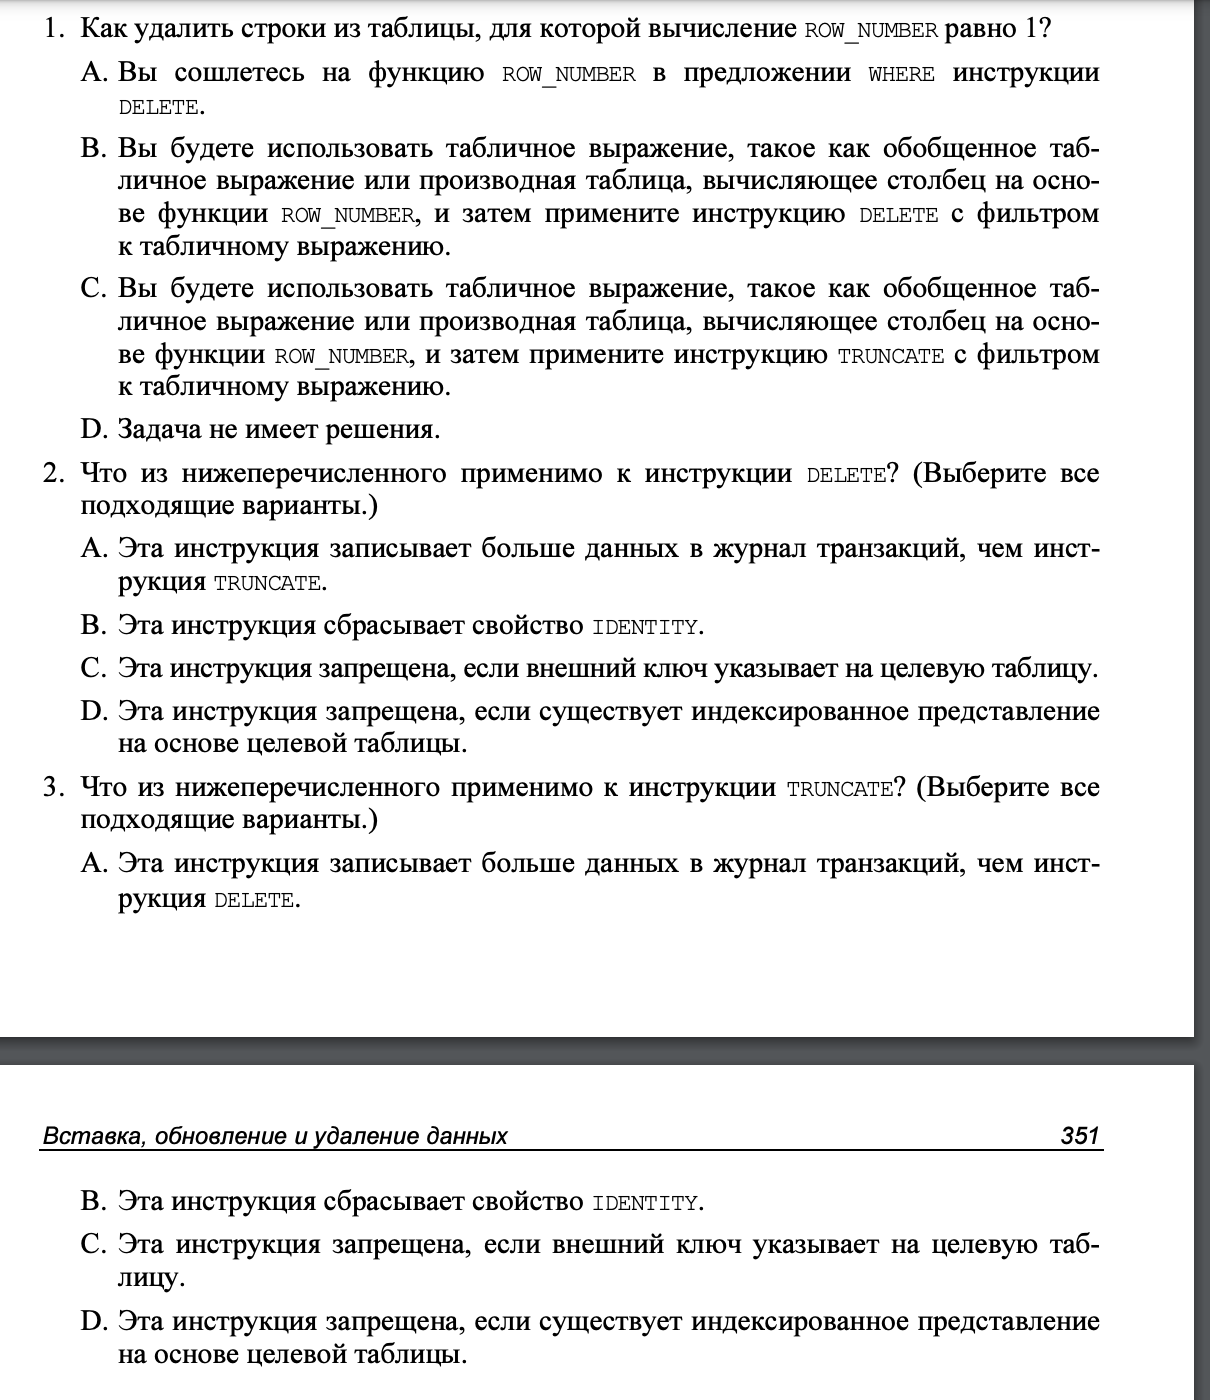
\includegraphics[width=0.9\textwidth]{img/zakrep24.png}
	\end{center}
	\captionsetup{justification=centering}
\end{figure}
\clearpage

\subsection*{Ответы}

\begin{figure}[h!]
	\begin{center}
		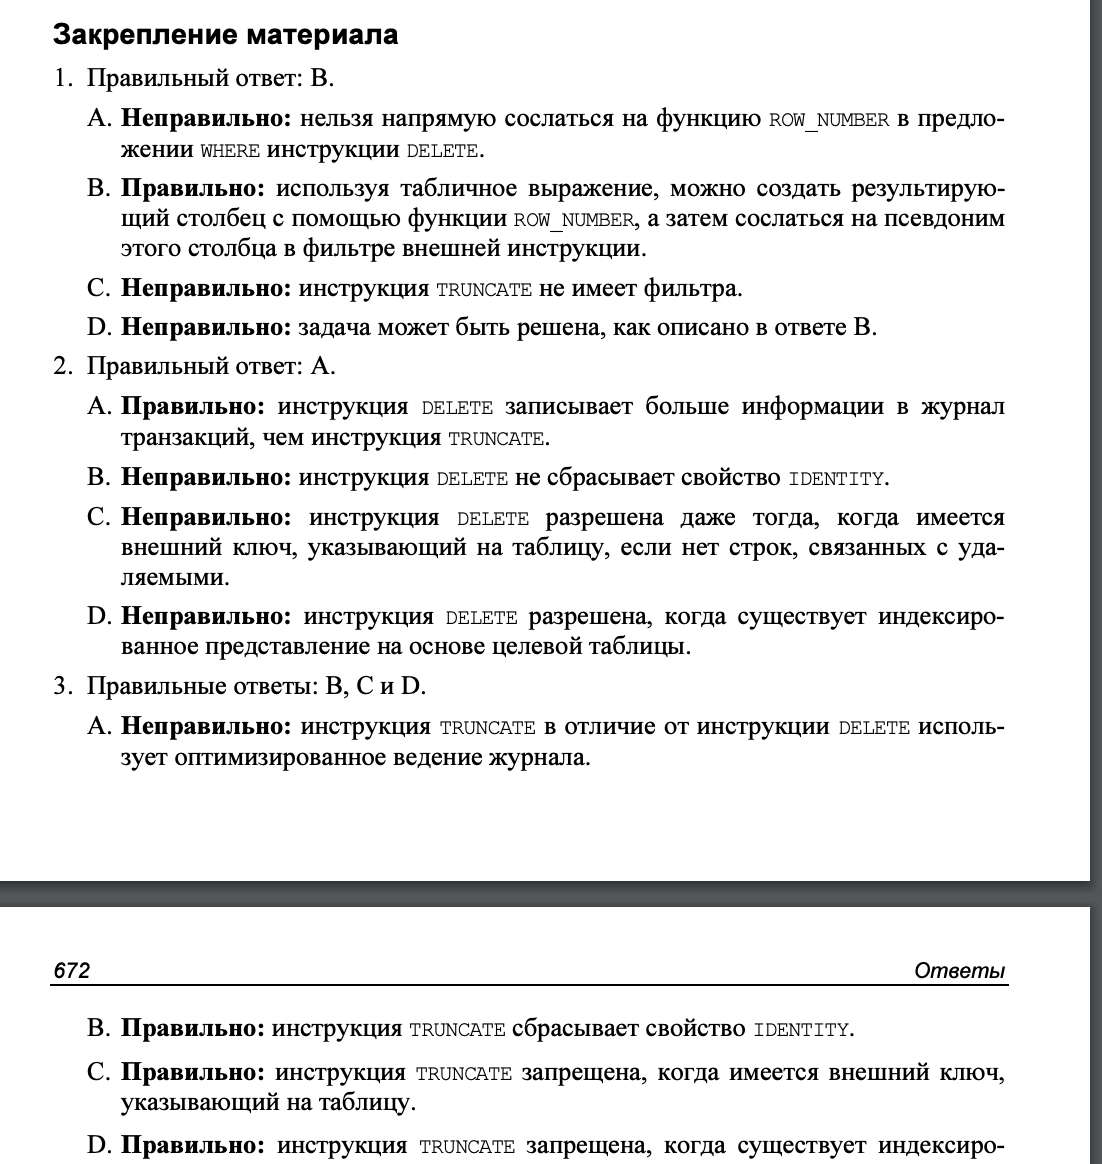
\includegraphics[width=0.8\textwidth]{img/ans23.png}
	\end{center}
	\captionsetup{justification=centering}
\end{figure}


\newpage
\subsection*{Упражнения}

\begin{figure}[h!]
	\begin{center}
		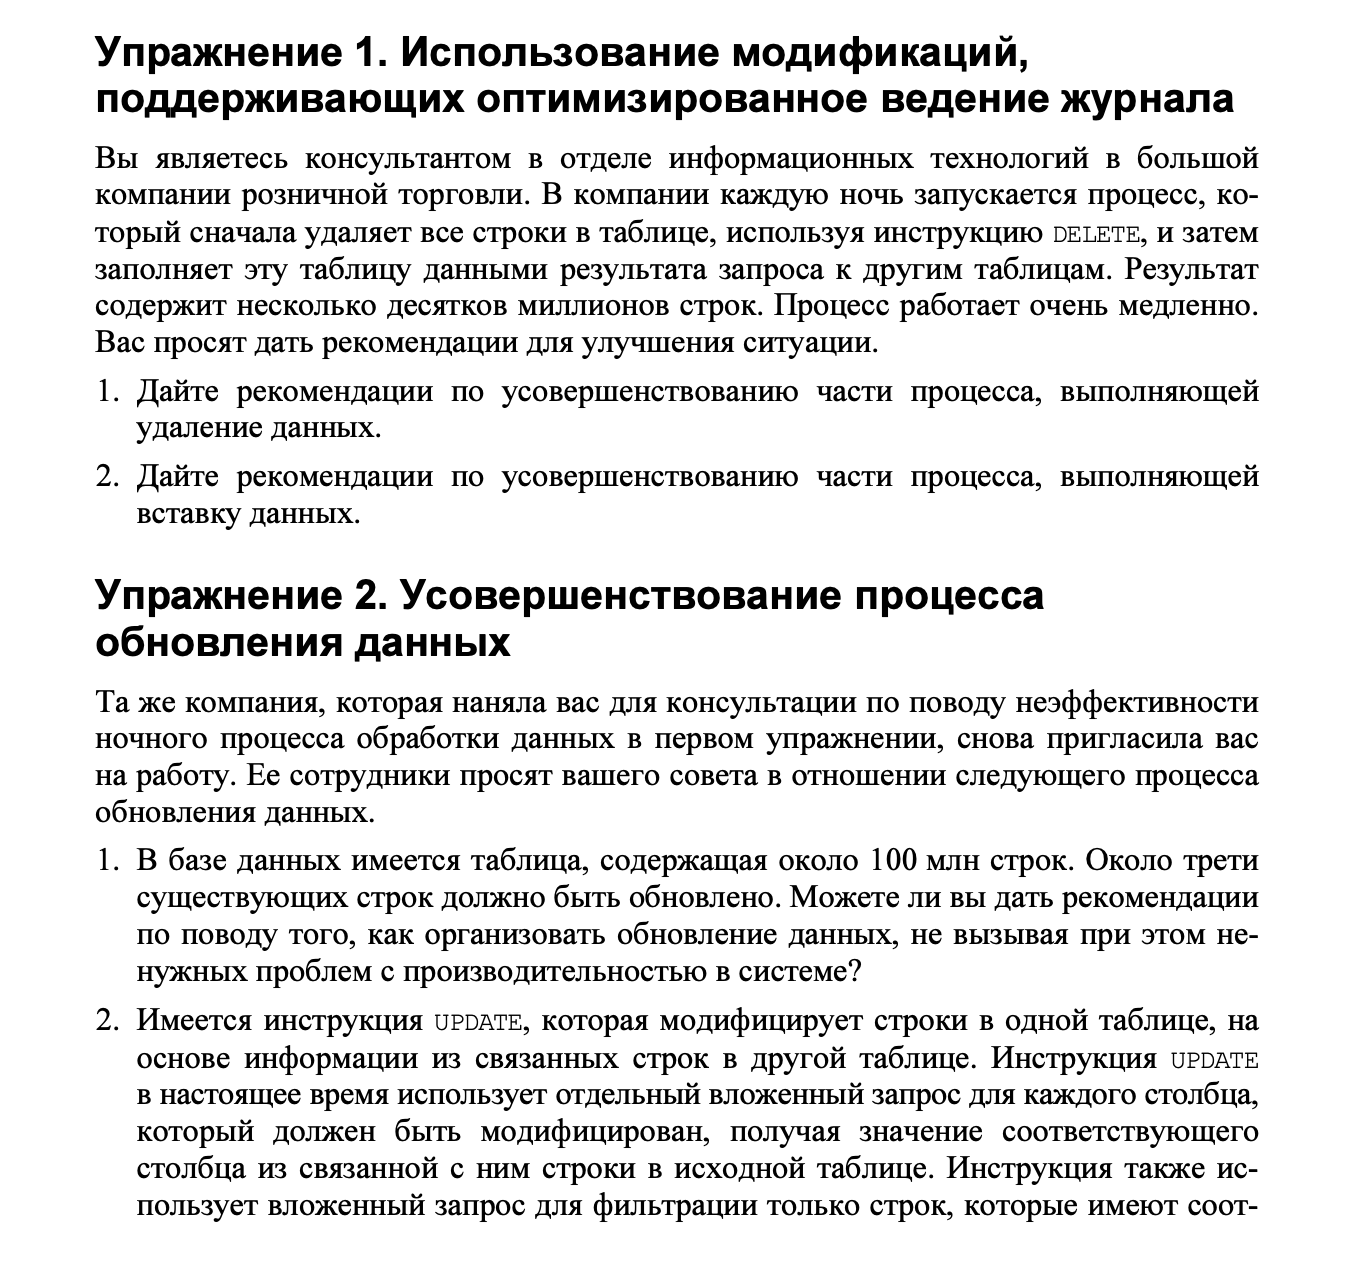
\includegraphics[width=0.9\textwidth]{img/ex16.png}
	\end{center}
	\captionsetup{justification=centering}
\end{figure}

\subsection*{Ответы}

\begin{figure}[h!]
	\begin{center}
		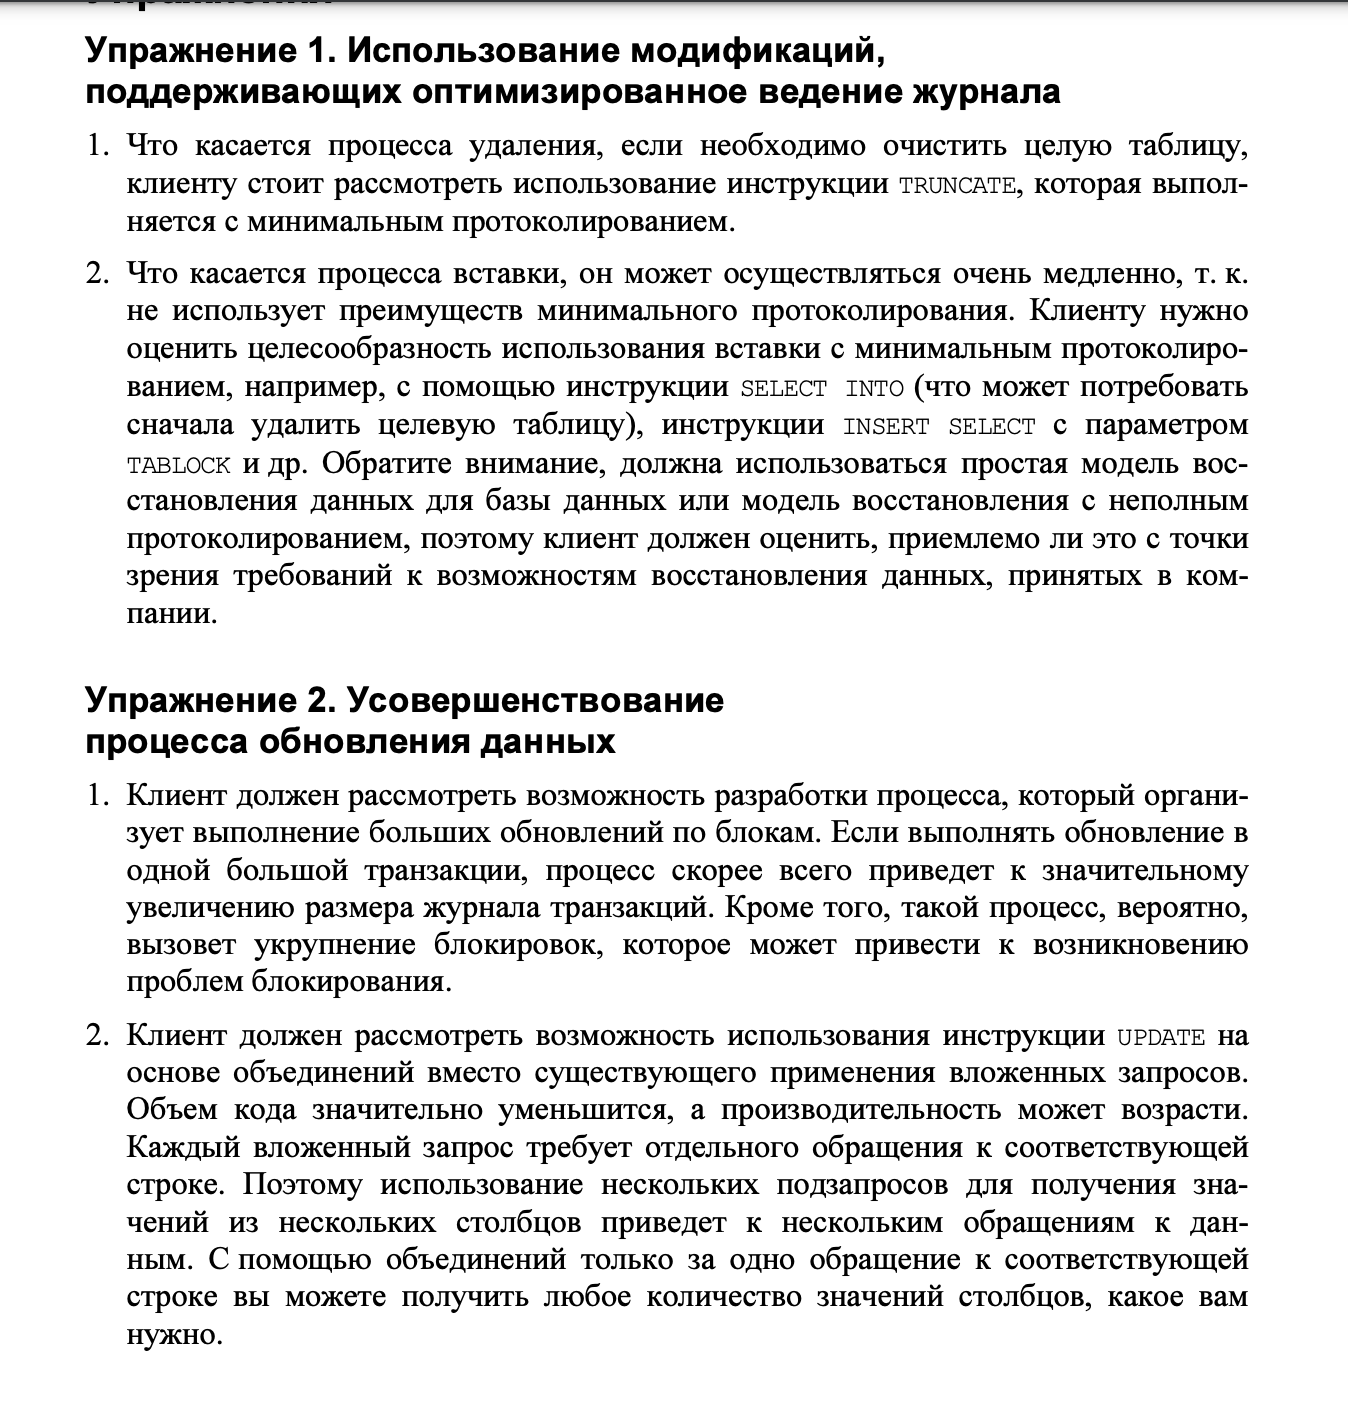
\includegraphics[width=0.9\textwidth]{img/eans16.png}
	\end{center}
	\captionsetup{justification=centering}
\end{figure}





